\begin{figure}[h]
\centering
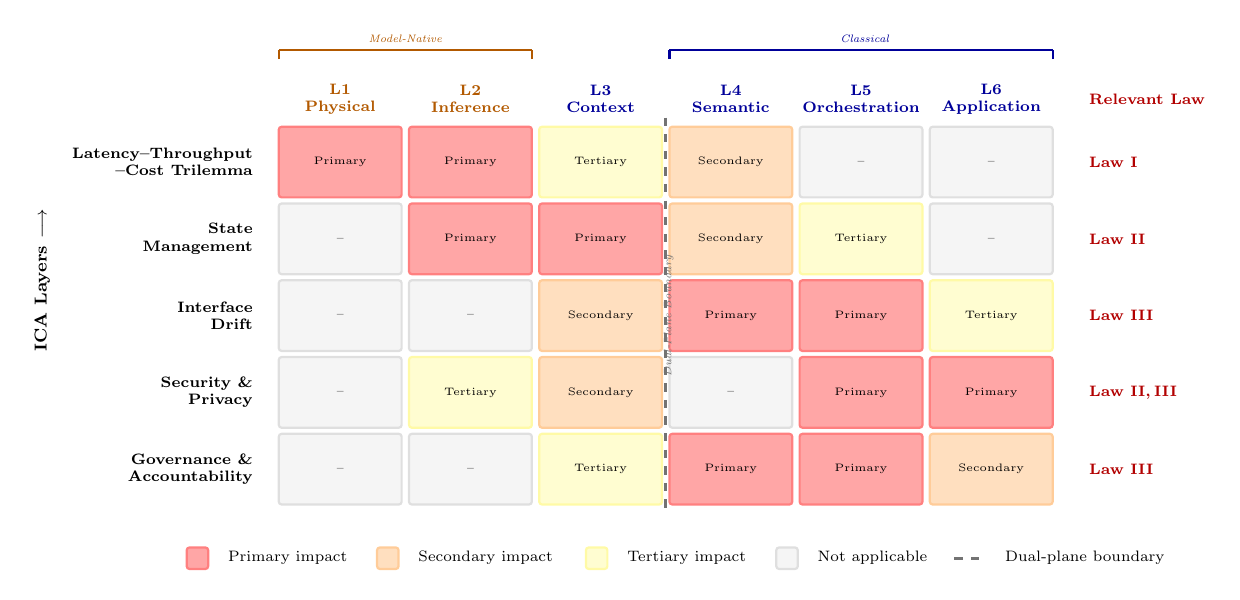
\begin{tikzpicture}[
    scale=0.78,
    transform shape,
    % --- cell styles by severity ---
    primary/.style={fill=red!35, draw=red!50, thick, rounded corners=1pt},
    secondary/.style={fill=orange!25, draw=orange!40, thick, rounded corners=1pt},
    tertiary/.style={fill=yellow!18, draw=yellow!35, thick, rounded corners=1pt},
    notapplic/.style={fill=gray!8, draw=gray!25, thick, rounded corners=1pt},
    % --- header styles ---
    colhead/.style={font=\scriptsize\bfseries, align=center, text width=1.8cm},
    rowhead/.style={font=\scriptsize\bfseries, align=right, anchor=east, text width=3.4cm},
    lawlabel/.style={font=\scriptsize\bfseries, align=center, anchor=west},
    celltxt/.style={font=\tiny, align=center},
    % --- axis labels ---
    axlbl/.style={font=\footnotesize\bfseries},
]

% === dimensions ===
\def\cellw{2.0}   % column width (cm)
\def\cellh{1.15}   % row height (cm)
\def\colsep{0.12}  % horizontal gap between cells
\def\rowsep{0.10}  % vertical gap between cells
\def\rowoff{5}     % number of rows minus 1 (0-indexed)
\def\coloff{5}     % number of cols minus 1 (0-indexed)

% === origin offsets ===
\def\xstart{4.0}   % left edge of first data column
\def\ystart{6.2}    % top edge of first data row

% === column headers (L1--L6) ===
% Use explicit two-line labels to prevent word-break hyphenation
\pgfmathsetmacro{\cx}{\xstart + 0*(\cellw+\colsep) + \cellw/2}
\node[colhead, text=orange!70!black] at (\cx, \ystart + 0.45) {L1\\Physical};
\pgfmathsetmacro{\cx}{\xstart + 1*(\cellw+\colsep) + \cellw/2}
\node[colhead, text=orange!70!black] at (\cx, \ystart + 0.45) {L2\\Inference};
\pgfmathsetmacro{\cx}{\xstart + 2*(\cellw+\colsep) + \cellw/2}
\node[colhead, text=blue!60!black] at (\cx, \ystart + 0.45) {L3\\Context};
\pgfmathsetmacro{\cx}{\xstart + 3*(\cellw+\colsep) + \cellw/2}
\node[colhead, text=blue!60!black] at (\cx, \ystart + 0.45) {L4\\Semantic};
\pgfmathsetmacro{\cx}{\xstart + 4*(\cellw+\colsep) + \cellw/2}
\node[font=\scriptsize\bfseries, align=center, text width=2.2cm, text=blue!60!black] at (\cx, \ystart + 0.45) {L5\\Orchestration};
\pgfmathsetmacro{\cx}{\xstart + 5*(\cellw+\colsep) + \cellw/2}
\node[colhead, text=blue!60!black] at (\cx, \ystart + 0.45) {L6\\Application};

% === column sub-headers: plane labels (raised slightly) ===
\pgfmathsetmacro{\modelnativex}{\xstart + \cellw + \colsep/2}
\node[font=\tiny\itshape, orange!70!black, anchor=south] at (\modelnativex, \ystart + 1.25) {Model-Native};
\pgfmathsetmacro{\classicalx}{\xstart + 3*(\cellw+\colsep) + 1.5*\cellw + 1.5*\colsep}
\node[font=\tiny\itshape, blue!60!black, anchor=south] at (\classicalx, \ystart + 1.25) {Classical};

% === row headers (5 challenges) ===
\pgfmathsetmacro{\rx}{\xstart - 0.3}
\pgfmathsetmacro{\ryA}{\ystart - 0*(\cellh+\rowsep) - \cellh/2}
\pgfmathsetmacro{\ryB}{\ystart - 1*(\cellh+\rowsep) - \cellh/2}
\pgfmathsetmacro{\ryC}{\ystart - 2*(\cellh+\rowsep) - \cellh/2}
\pgfmathsetmacro{\ryD}{\ystart - 3*(\cellh+\rowsep) - \cellh/2}
\pgfmathsetmacro{\ryE}{\ystart - 4*(\cellh+\rowsep) - \cellh/2}
\node[rowhead] at (\rx, \ryA)
    {Latency--Throughput\\--Cost Trilemma};
\node[rowhead] at (\rx, \ryB)
    {State\\Management};
\node[rowhead] at (\rx, \ryC)
    {Interface\\Drift};
\node[rowhead] at (\rx, \ryD)
    {Security \&\\Privacy};
\node[rowhead] at (\rx, \ryE)
    {Governance \&\\Accountability};

% === heatmap cells ===
% Row 0: Latency/Cost -- Primary L1,L2; Secondary L4; Tertiary L3; NA L5,L6
\foreach \c/\sty in {0/primary, 1/primary, 2/tertiary, 3/secondary, 4/notapplic, 5/notapplic}{
    \pgfmathsetmacro{\xll}{\xstart + \c*(\cellw+\colsep)}
    \pgfmathsetmacro{\yll}{\ystart - \cellh}
    \draw[\sty] (\xll, \yll) rectangle +(\cellw, \cellh);
}
% Severity text inside cells
\foreach \c/\lab in {0/Primary, 1/Primary, 2/Tertiary, 3/Secondary, 4/--, 5/--}{
    \pgfmathsetmacro{\cx}{\xstart + \c*(\cellw+\colsep) + \cellw/2}
    \pgfmathsetmacro{\cy}{\ystart - \cellh + \cellh/2}
    \node[celltxt] at (\cx, \cy) {\lab};
}

% Row 1: State Mgmt -- Primary L2,L3; Secondary L4; Tertiary L5; NA L1,L6
\foreach \c/\sty in {0/notapplic, 1/primary, 2/primary, 3/secondary, 4/tertiary, 5/notapplic}{
    \pgfmathsetmacro{\xll}{\xstart + \c*(\cellw+\colsep)}
    \pgfmathsetmacro{\yll}{\ystart - 1*(\cellh+\rowsep) - \cellh}
    \draw[\sty] (\xll, \yll) rectangle +(\cellw, \cellh);
}
\foreach \c/\lab in {0/--, 1/Primary, 2/Primary, 3/Secondary, 4/Tertiary, 5/--}{
    \pgfmathsetmacro{\cx}{\xstart + \c*(\cellw+\colsep) + \cellw/2}
    \pgfmathsetmacro{\cy}{\ystart - 1*(\cellh+\rowsep) - \cellh + \cellh/2}
    \node[celltxt] at (\cx, \cy) {\lab};
}

% Row 2: Interface Drift -- Primary L4,L5; Secondary L3; Tertiary L6; NA L1,L2
\foreach \c/\sty in {0/notapplic, 1/notapplic, 2/secondary, 3/primary, 4/primary, 5/tertiary}{
    \pgfmathsetmacro{\xll}{\xstart + \c*(\cellw+\colsep)}
    \pgfmathsetmacro{\yll}{\ystart - 2*(\cellh+\rowsep) - \cellh}
    \draw[\sty] (\xll, \yll) rectangle +(\cellw, \cellh);
}
\foreach \c/\lab in {0/--, 1/--, 2/Secondary, 3/Primary, 4/Primary, 5/Tertiary}{
    \pgfmathsetmacro{\cx}{\xstart + \c*(\cellw+\colsep) + \cellw/2}
    \pgfmathsetmacro{\cy}{\ystart - 2*(\cellh+\rowsep) - \cellh + \cellh/2}
    \node[celltxt] at (\cx, \cy) {\lab};
}

% Row 3: Security & Privacy -- Primary L5,L6; Secondary L3; Tertiary L2; NA L1,L4
\foreach \c/\sty in {0/notapplic, 1/tertiary, 2/secondary, 3/notapplic, 4/primary, 5/primary}{
    \pgfmathsetmacro{\xll}{\xstart + \c*(\cellw+\colsep)}
    \pgfmathsetmacro{\yll}{\ystart - 3*(\cellh+\rowsep) - \cellh}
    \draw[\sty] (\xll, \yll) rectangle +(\cellw, \cellh);
}
\foreach \c/\lab in {0/--, 1/Tertiary, 2/Secondary, 3/--, 4/Primary, 5/Primary}{
    \pgfmathsetmacro{\cx}{\xstart + \c*(\cellw+\colsep) + \cellw/2}
    \pgfmathsetmacro{\cy}{\ystart - 3*(\cellh+\rowsep) - \cellh + \cellh/2}
    \node[celltxt] at (\cx, \cy) {\lab};
}

% Row 4: Governance -- Primary L4,L5; Secondary L6; Tertiary L3; NA L1,L2
\foreach \c/\sty in {0/notapplic, 1/notapplic, 2/tertiary, 3/primary, 4/primary, 5/secondary}{
    \pgfmathsetmacro{\xll}{\xstart + \c*(\cellw+\colsep)}
    \pgfmathsetmacro{\yll}{\ystart - 4*(\cellh+\rowsep) - \cellh}
    \draw[\sty] (\xll, \yll) rectangle +(\cellw, \cellh);
}
\foreach \c/\lab in {0/--, 1/--, 2/Tertiary, 3/Primary, 4/Primary, 5/Secondary}{
    \pgfmathsetmacro{\cx}{\xstart + \c*(\cellw+\colsep) + \cellw/2}
    \pgfmathsetmacro{\cy}{\ystart - 4*(\cellh+\rowsep) - \cellh + \cellh/2}
    \node[celltxt] at (\cx, \cy) {\lab};
}

% === Dual-plane boundary: thick dashed line between L3 and L4 ===
\pgfmathsetmacro{\bndx}{\xstart + 3*(\cellw+\colsep) - \colsep/2}
\pgfmathsetmacro{\bndtop}{\ystart + 0.15}
\pgfmathsetmacro{\bndbot}{\ystart - 4*(\cellh+\rowsep) - \cellh - 0.15}
\draw[very thick, dashed, black!55] (\bndx, \bndtop) -- (\bndx, \bndbot);

% Small label for the boundary
\pgfmathsetmacro{\bndmid}{(\bndtop + \bndbot)/2}
\node[font=\tiny\itshape, black!55, rotate=90, anchor=south] at (\bndx + 0.25, \bndmid)
    {Dual-Plane Boundary};

% === Right-margin annotation: quantitative law relevance ===
\pgfmathsetmacro{\lawx}{\xstart + 6*(\cellw+\colsep) + 0.35}

% Row 0: Latency/Cost -> Law I (Energy/Performance scaling)
\pgfmathsetmacro{\ry}{\ystart - 0*(\cellh+\rowsep) - \cellh/2}
\node[lawlabel, red!70!black] at (\lawx, \ry) {Law~I};

% Row 1: State Mgmt -> Law II (Memory/State consistency)
\pgfmathsetmacro{\ry}{\ystart - 1*(\cellh+\rowsep) - \cellh/2}
\node[lawlabel, red!70!black] at (\lawx, \ry) {Law~II};

% Row 2: Interface Drift -> Law III (Interface stability)
\pgfmathsetmacro{\ry}{\ystart - 2*(\cellh+\rowsep) - \cellh/2}
\node[lawlabel, red!70!black] at (\lawx, \ry) {Law~III};

% Row 3: Security & Privacy -> Law III + II
\pgfmathsetmacro{\ry}{\ystart - 3*(\cellh+\rowsep) - \cellh/2}
\node[lawlabel, red!70!black] at (\lawx, \ry) {Law~II,\,III};

% Row 4: Governance -> Law III
\pgfmathsetmacro{\ry}{\ystart - 4*(\cellh+\rowsep) - \cellh/2}
\node[lawlabel, red!70!black] at (\lawx, \ry) {Law~III};

% Right-margin column header
\node[font=\scriptsize\bfseries, red!70!black, anchor=west] at (\lawx, \ystart + 0.45)
    {Relevant Law};

% === Axis labels ===
\pgfmathsetmacro{\axleft}{\xstart - 3.6}
\pgfmathsetmacro{\axmid}{\ystart - 2*(\cellh+\rowsep)}
\node[axlbl, rotate=90, anchor=south] at (\axleft, \axmid)
    {ICA Layers $\longrightarrow$};

\pgfmathsetmacro{\axbotx}{\xstart + 2.5*(\cellw+\colsep)}
\pgfmathsetmacro{\axboty}{\ystart - 4*(\cellh+\rowsep) - \cellh - 0.5}
\node[axlbl, anchor=north] at (\axbotx, \axboty) {};

% === Legend (centred, items spaced so text doesn't overlap next box) ===
\def\legy{-1.0}
\def\legx{2.5}
% Each item: box(0.35) + gap(0.2) + text + gap(0.5) before next box
% "Primary impact" ~1.8cm, "Secondary impact" ~2.1cm, "Tertiary impact" ~1.7cm
% item spacing: 3.1cm apart

% Primary
\draw[primary] (\legx, \legy) rectangle +(0.35, 0.35);
\node[font=\scriptsize, anchor=west] at (\legx + 0.55, \legy + 0.175)
    {Primary impact\hspace{0.4em}};

% Secondary  (start at legx + 3.1)
\pgfmathsetmacro{\lx}{\legx + 3.1}
\draw[secondary] (\lx, \legy) rectangle +(0.35, 0.35);
\node[font=\scriptsize, anchor=west] at (\lx + 0.55, \legy + 0.175)
    {Secondary impact\hspace{0.4em}};

% Tertiary  (start at legx + 6.5)
\pgfmathsetmacro{\lx}{\legx + 6.5}
\draw[tertiary] (\lx, \legy) rectangle +(0.35, 0.35);
\node[font=\scriptsize, anchor=west] at (\lx + 0.55, \legy + 0.175)
    {Tertiary impact\hspace{0.4em}};

% Not applicable  (start at legx + 9.6)
\pgfmathsetmacro{\lx}{\legx + 9.6}
\draw[notapplic] (\lx, \legy) rectangle +(0.35, 0.35);
\node[font=\scriptsize, anchor=west] at (\lx + 0.55, \legy + 0.175)
    {Not applicable\hspace{0.4em}};

% Boundary legend entry  (start at legx + 12.5)
\pgfmathsetmacro{\lx}{\legx + 12.5}
\draw[very thick, dashed, black!55] (\lx, \legy + 0.175) -- ++(0.5, 0);
\node[font=\scriptsize, anchor=west] at (\lx + 0.7, \legy + 0.175)
    {Dual-plane boundary};

% Plane annotations along top
\pgfmathsetmacro{\modelleft}{\xstart}
\pgfmathsetmacro{\modelright}{\xstart + 2*\cellw + \colsep}
\pgfmathsetmacro{\classleft}{\xstart + 3*(\cellw+\colsep)}
\pgfmathsetmacro{\classright}{\xstart + 5*(\cellw+\colsep) + \cellw}
\pgfmathsetmacro{\bracetop}{\ystart + 1.1}

% Underbrace for model-native plane
\draw[thick, orange!70!black]
    (\modelleft, \bracetop) -- (\modelleft, \bracetop + 0.15);
\draw[thick, orange!70!black]
    (\modelright, \bracetop) -- (\modelright, \bracetop + 0.15);
\draw[thick, orange!70!black]
    (\modelleft, \bracetop + 0.15) -- (\modelright, \bracetop + 0.15);

% Underbrace for classical plane
\draw[thick, blue!60!black]
    (\classleft, \bracetop) -- (\classleft, \bracetop + 0.15);
\draw[thick, blue!60!black]
    (\classright, \bracetop) -- (\classright, \bracetop + 0.15);
\draw[thick, blue!60!black]
    (\classleft, \bracetop + 0.15) -- (\classright, \bracetop + 0.15);

\end{tikzpicture}
\caption{Challenge-to-ICA-layer impact heatmap. Each cell indicates the severity of a given challenge at the corresponding ICA layer: \textcolor{red!50}{\textbf{primary}} (direct, critical impact), \textcolor{orange!40}{\textbf{secondary}} (significant but indirect), \textcolor{yellow!50!black}{\textbf{tertiary}} (moderate, contextual), or \textcolor{gray!40}{not applicable}. The thick dashed line marks the dual-plane boundary between model-native layers (L1--L2) and classical layers (L3--L6). The right-margin column identifies the most relevant quantitative law for each challenge row.}
\label{fig:challenge_heatmap}
\end{figure}
